\documentclass{article}
\usepackage{tikz}
\usetikzlibrary{automata,positioning}

\begin{document}

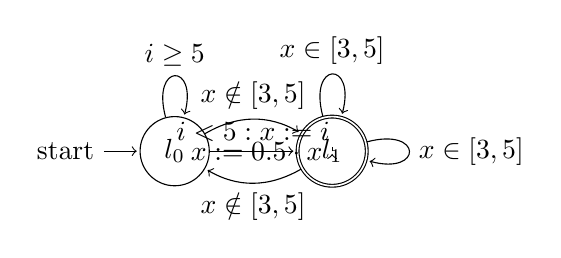
\begin{tikzpicture}[shorten >=1pt,node distance=2cm,on grid,auto]
    \node[state,initial] (l0) {$l_0$};
    \node[state,accepting] (l1) [right=of l0] {$l_1$};

    \path[->]
        (l0) edge [loop above] node {$i \geq 5$} ()
             edge [bend left] node {$x \notin [3,5]$} (l1)
        (l1) edge [loop above] node {$x \in [3,5]$} ()
             edge [bend left] node {$x \notin [3,5]$} (l0)
             edge [loop right] node {$x \in [3,5]$} ();
    \path[->]
        (l0) edge node {$i < 5 : x := i$} (l1);
    \path[->]
        (l1) edge node {$x := 0.5 \cdot x$} (l1);
\end{tikzpicture}

\end{document}